\subsection{Augmentacja}

Po stworzeniu potoku przyszedł czas na zaprojektowanie mechanizmów zwielokrotniających dane treningowe (ang. \textit{data augmentation}). W~pierwszej kolejności należało wybrać pomiędzy podejściem \textit{online} a~\textit{offline}. Pierwsze z~nich polega na generowaniu losowych modyfikacji danych wejściowych na bieżąco \underline{w~trakcie trwania} trening. Z~kolei drugie zakłada wygenerowanie zwielokrotnionego zbioru treningowego o~określonej wielkości \underline{przed} przystąpieniem do treningu. Ze względu na wygodę użytkowania i~przekazywania tworzonego pakietu oprogramowania pomiędzy członkami grupy zdecydowano się na wariant pierwszy.

Interfejs \textit{tf.data} dostarcza wygodny sposób nakładania arbitralnych modyfikacji na dane przepływające przez potok. Jak opisano wcześniej iniekcja transformacji ma miejsce przed etapem podziału danych na porcje. Aby zapewnić odpowiednią elastyczność decyzji postanowiono zaimplementować szereg mechanizmów augmentacji, z~których po przeprowadzeniu pobieżnego badania ich efektywności tylko cześć miała zostać wykorzystana. Rozwiązanie ponownie zamknięto w~postaci klasy parametryzowalnej z~poziomu plików konfiguracyjnych. Udostępnia ona następujące transformacje obrazów wejściowych:

\begin{itemize}
    \setlength\itemsep{0.3em}
    \item losowe korekcje jasności
    \item losowe korekcje kontrastu
    \item losowe odbicia lustrzane względem osi X~i~Y
    \item losowe przybliżenia
    \item losowe rotacje
    \item losowe przesunięcia wzdłuż osi X~i~Y
    \item losowe transformacje typu \textit{shear} wzdłuż osi X~i~Y
\end{itemize}

Wszystkie wartości losuje się z~rozkładów jednostajnych, których granice można skonfigurować przed treningiem. Puste piksele powstałe na skutek modyfikacji są wypełniane kolorem białym stanowiącym domyślne tło we wszystkich zdjęciach. Ramy czasowe projektu nie pozwoliły na gruntowne przebadanie wpływu transformacji na wyniki uczonych sieci. Posiłkując się drobnymi testami oraz analizą charakteru zbioru danych zdecydowano się na wykorzystanie odbić lustrzanych względem osi X~i~Y oraz rotacji o~kąt z~przedziału $[-20^{\circ}; 20^{\circ}]$  (kolejność zgodna z~porządkiem aplikowania). Należy zaznaczyć, że transformacje te były niezmienne na przestrzeni wszystkich przeprowadzonych w~czasie projektu treningów.

\vspace{0.5cm}
\begin{figure}[h]
    \centering
    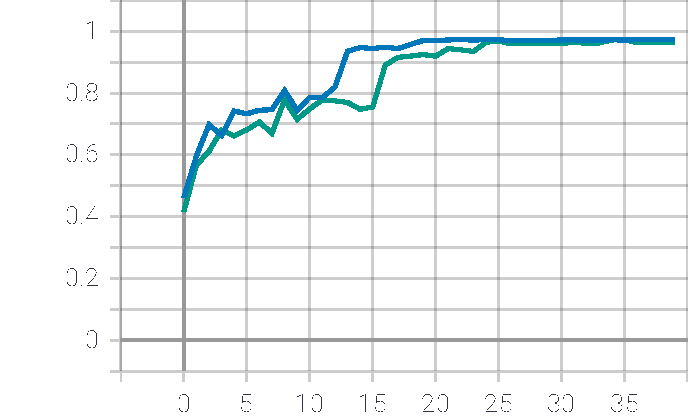
\includegraphics[scale=0.8]{img/eugmentation_test.pdf}
    \captionsetup{format=plain,justification=centering}
    \caption{\small Porównanie mechanizmów zwielokrotniania danych na przykładzie uczenia części perceptronowej wraz z~dwiema ostatnimi warstwami konwolucyjnymi. Widać, że w~przypadku przyjętego zbioru transformacji (na niebiesko) dokładność na zbiorze walidacyjnym rośnie szybciej niż w~przypadku dodania losowych korekcji jasności i~kontrastu (na zielono).}
    \label{augmentation_test_img}
\end{figure}
\vspace{0.5cm}



